\documentclass[11pt]{article}
\usepackage[textwidth=18.0cm, textheight=23.0cm, top=2.0cm]{geometry}
\usepackage{pst-all}
\usepackage{amssymb}
\usepackage{tikz}
\usepackage{underscore}\begin{document}
\pagestyle{empty}


ClassName: \underline{\textbf{Class_10.2bp-16}}
\par
BinSize: \underline{\textbf{100 × 100}}
\par
ReduceSize: \underline{\textbf{100 × 100}}
\par
TypeNum: \underline{\textbf{40}}
\par
Num: \underline{\textbf{40}}
\par
OutS: \underline{\textbf{70000}}
\par
InS: \underline{\textbf{60834}}
\par
Rate: \underline{\textbf{0.869}}
\par
UB: \underline{\textbf{7}}
\par
LB0: \underline{\textbf{7}}
\par
LB: \underline{\textbf{7}}
\par
LBWithCut: \underline{\textbf{7}}
\par
NodeCut: \underline{\textbf{0}}
\par
ExtendedNodeCnt: \underline{\textbf{1}}
\par
GenNodeCnt: \underline{\textbf{1}}
\par
PrimalNode: \underline{\textbf{0}}
\par
ColumnCount: \underline{\textbf{7}}
\par
TotalCutCount: \underline{\textbf{0}}
\par
RootCutCount: \underline{\textbf{0}}
\par
LPSolverCnt: \underline{\textbf{1}}
\par
PricingSolverCnt: \underline{\textbf{0}}
\par
BranchAndBoundNum: \underline{\textbf{1}}
\par
isOpt: \underline{\textbf{true}}
\par
TimeOnPrimal: \underline{\textbf{0.000 s}}
\par
TimeOnPricing: \underline{\textbf{0.000 s}}
\par
TimeOnRmp: \underline{\textbf{0.063 s}}
\par
TotalTime: \underline{\textbf{0.125 s}}
\par
\newpage


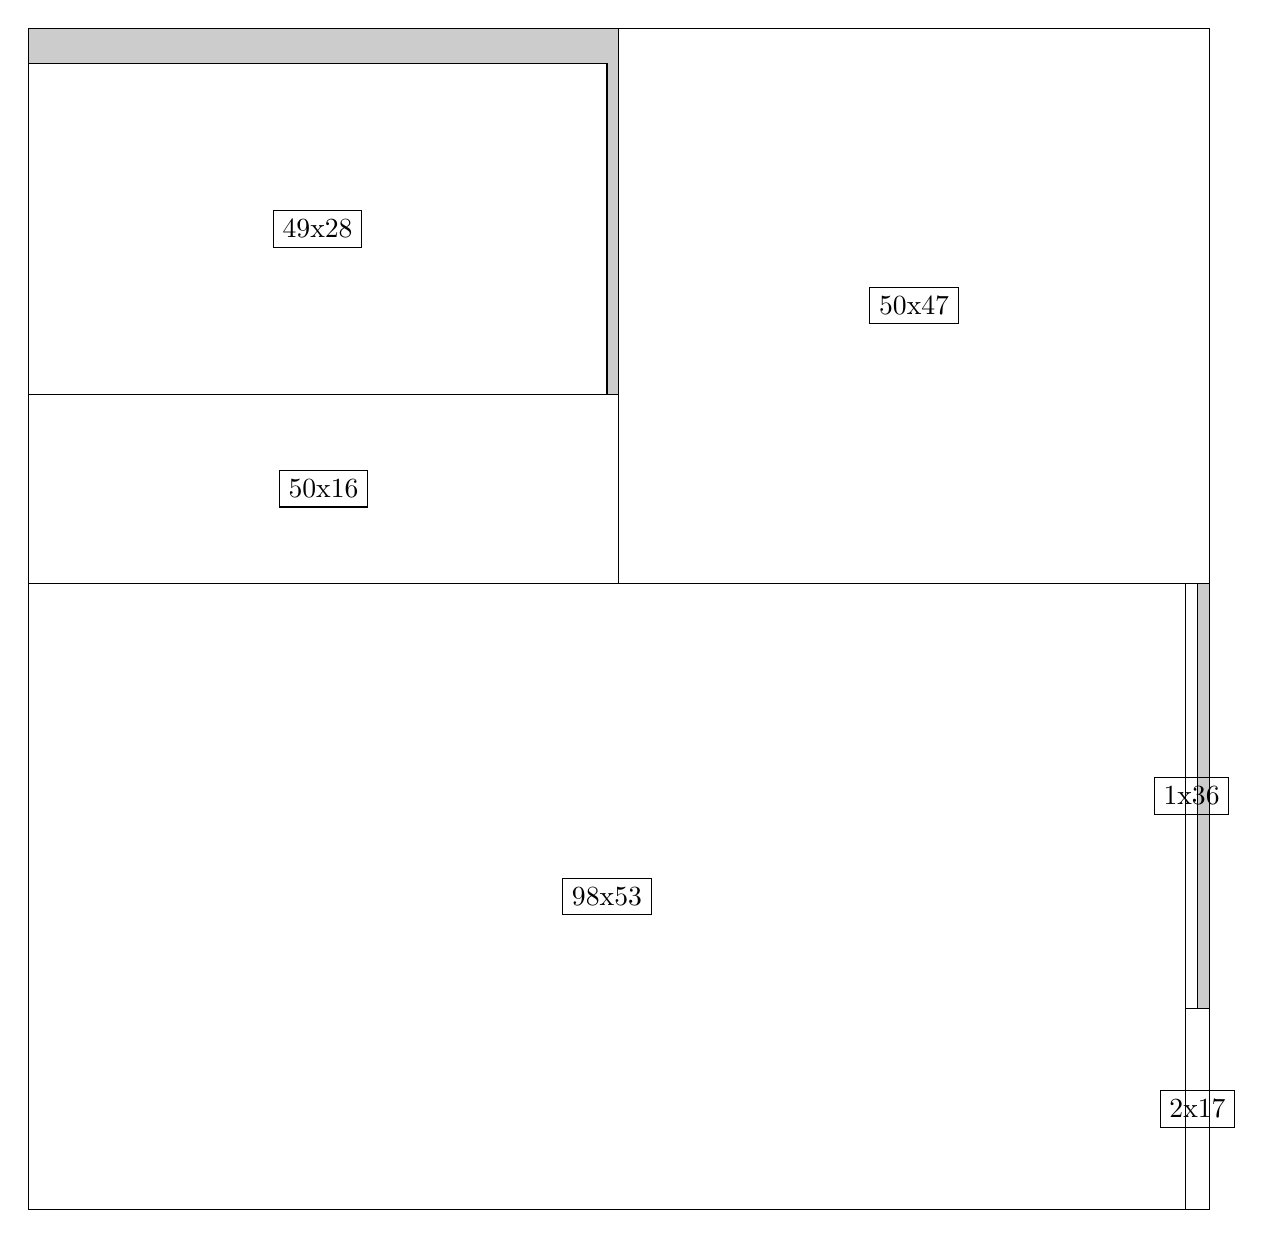
\begin{tikzpicture}[shorten >=1pt,scale=1.0,every node/.style={scale=1.0},->]
\tikzstyle{vertex}=[circle,fill=black!25,minimum size=14pt,inner sep=0pt]
\filldraw[fill=gray!40!white, draw=black] (0,0) rectangle (15.0,15.0);
\foreach \name/\x/\y/\w/\h in {98x53/0.0/0.0/14.7/7.949999999999999,50x47/7.5/7.949999999999999/7.5/7.05,50x16/0.0/7.949999999999999/7.5/2.4,49x28/0.0/10.35/7.35/4.2,1x36/14.7/2.55/0.15/5.3999999999999995,2x17/14.7/0.0/0.3/2.55}
\filldraw[fill=white!40!white, draw=black] (\x,\y) rectangle node[draw] (\name) {\name} ++(\w,\h);
\end{tikzpicture}


w =98 , h =53 , x =0 , y =0 , v =5194
\par
w =50 , h =47 , x =50 , y =53 , v =2350
\par
w =50 , h =16 , x =0 , y =53 , v =800
\par
w =49 , h =28 , x =0 , y =69 , v =1372
\par
w =1 , h =36 , x =98 , y =17 , v =36
\par
w =2 , h =17 , x =98 , y =0 , v =34
\par
\newpage


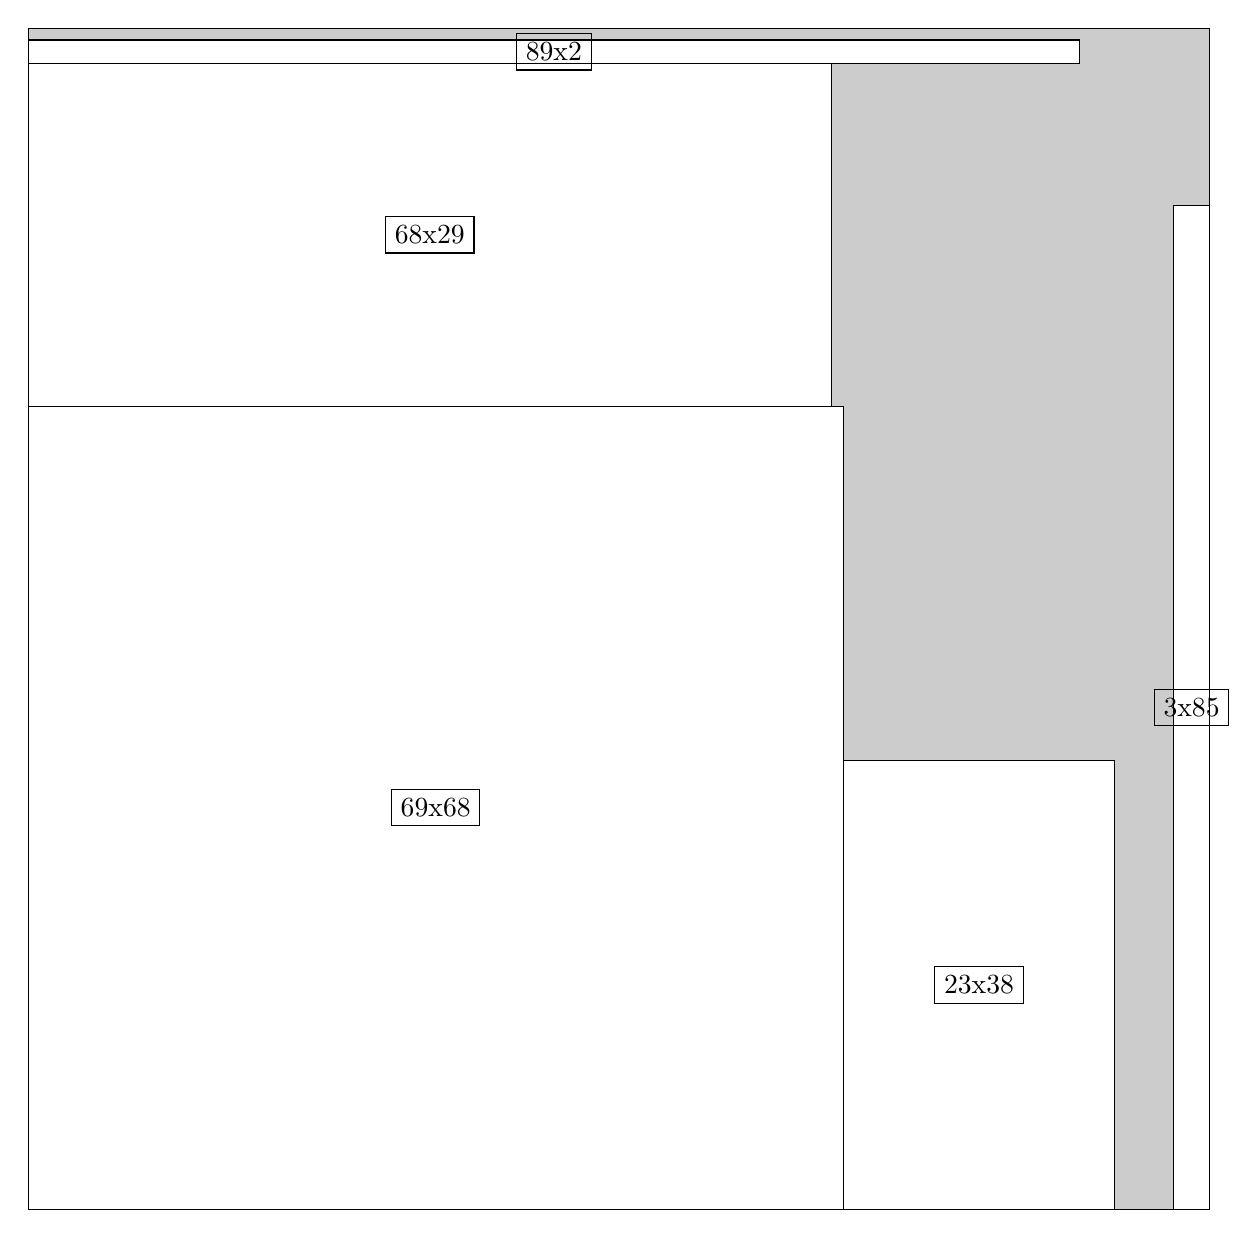
\begin{tikzpicture}[shorten >=1pt,scale=1.0,every node/.style={scale=1.0},->]
\tikzstyle{vertex}=[circle,fill=black!25,minimum size=14pt,inner sep=0pt]
\filldraw[fill=gray!40!white, draw=black] (0,0) rectangle (15.0,15.0);
\foreach \name/\x/\y/\w/\h in {69x68/0.0/0.0/10.35/10.2,68x29/0.0/10.2/10.2/4.35,23x38/10.35/0.0/3.4499999999999997/5.7,3x85/14.549999999999999/0.0/0.44999999999999996/12.75,89x2/0.0/14.549999999999999/13.35/0.3}
\filldraw[fill=white!40!white, draw=black] (\x,\y) rectangle node[draw] (\name) {\name} ++(\w,\h);
\end{tikzpicture}


w =69 , h =68 , x =0 , y =0 , v =4692
\par
w =68 , h =29 , x =0 , y =68 , v =1972
\par
w =23 , h =38 , x =69 , y =0 , v =874
\par
w =3 , h =85 , x =97 , y =0 , v =255
\par
w =89 , h =2 , x =0 , y =97 , v =178
\par
\newpage


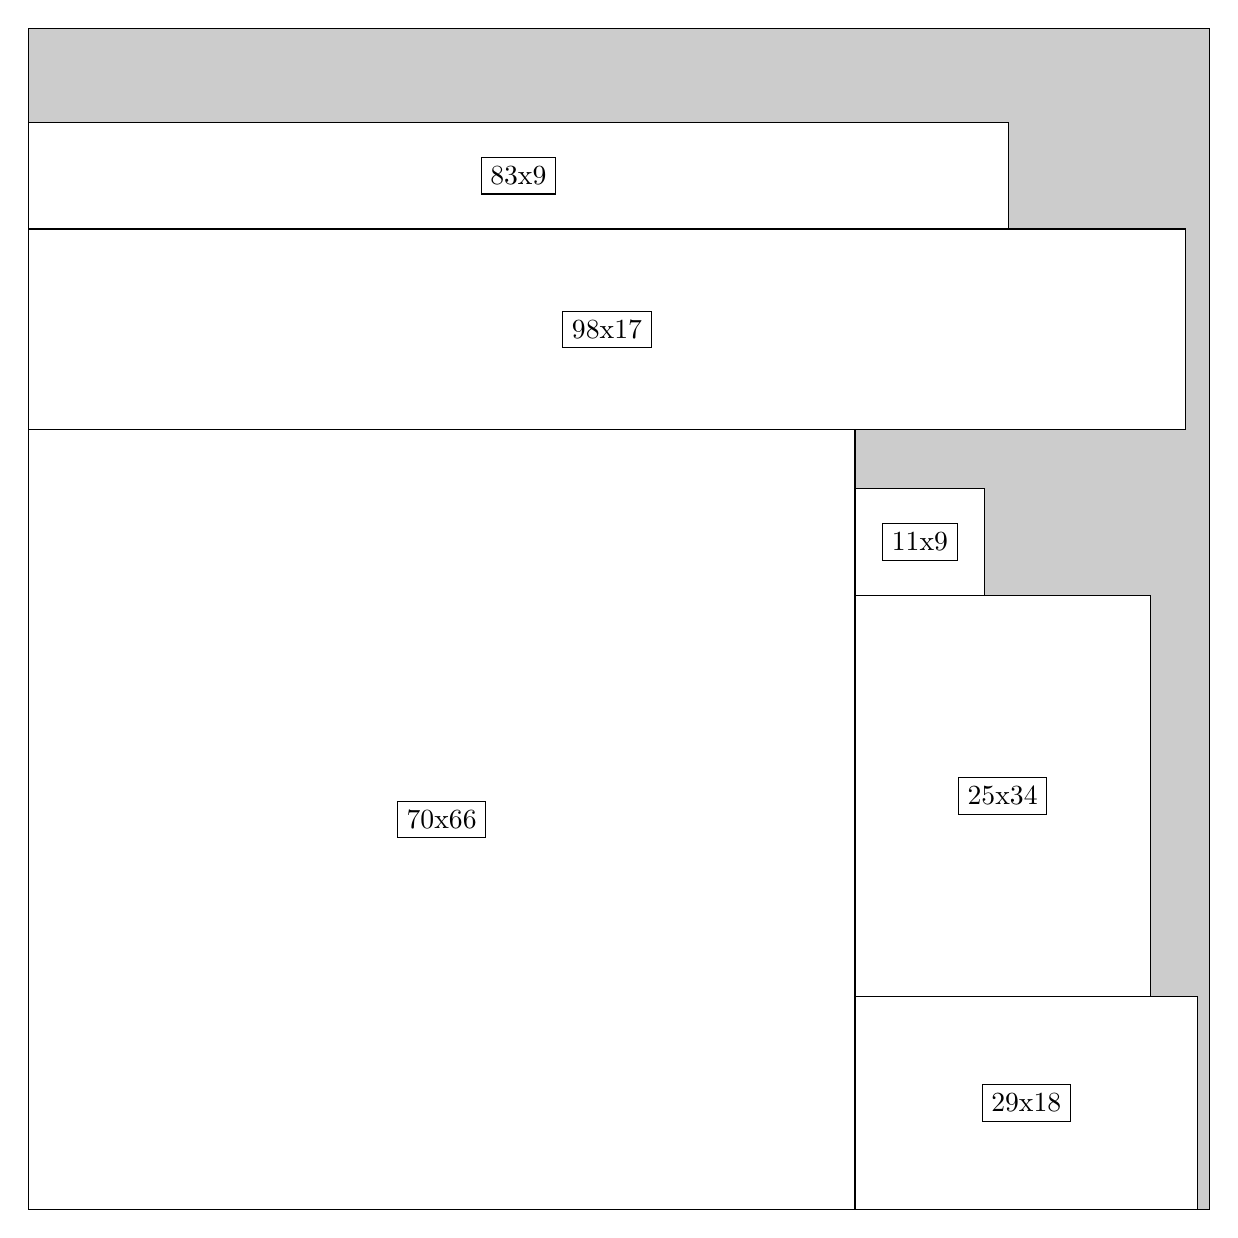
\begin{tikzpicture}[shorten >=1pt,scale=1.0,every node/.style={scale=1.0},->]
\tikzstyle{vertex}=[circle,fill=black!25,minimum size=14pt,inner sep=0pt]
\filldraw[fill=gray!40!white, draw=black] (0,0) rectangle (15.0,15.0);
\foreach \name/\x/\y/\w/\h in {70x66/0.0/0.0/10.5/9.9,98x17/0.0/9.9/14.7/2.55,25x34/10.5/2.6999999999999997/3.75/5.1,83x9/0.0/12.45/12.45/1.3499999999999999,29x18/10.5/0.0/4.35/2.6999999999999997,11x9/10.5/7.8/1.65/1.3499999999999999}
\filldraw[fill=white!40!white, draw=black] (\x,\y) rectangle node[draw] (\name) {\name} ++(\w,\h);
\end{tikzpicture}


w =70 , h =66 , x =0 , y =0 , v =4620
\par
w =98 , h =17 , x =0 , y =66 , v =1666
\par
w =25 , h =34 , x =70 , y =18 , v =850
\par
w =83 , h =9 , x =0 , y =83 , v =747
\par
w =29 , h =18 , x =70 , y =0 , v =522
\par
w =11 , h =9 , x =70 , y =52 , v =99
\par
\newpage


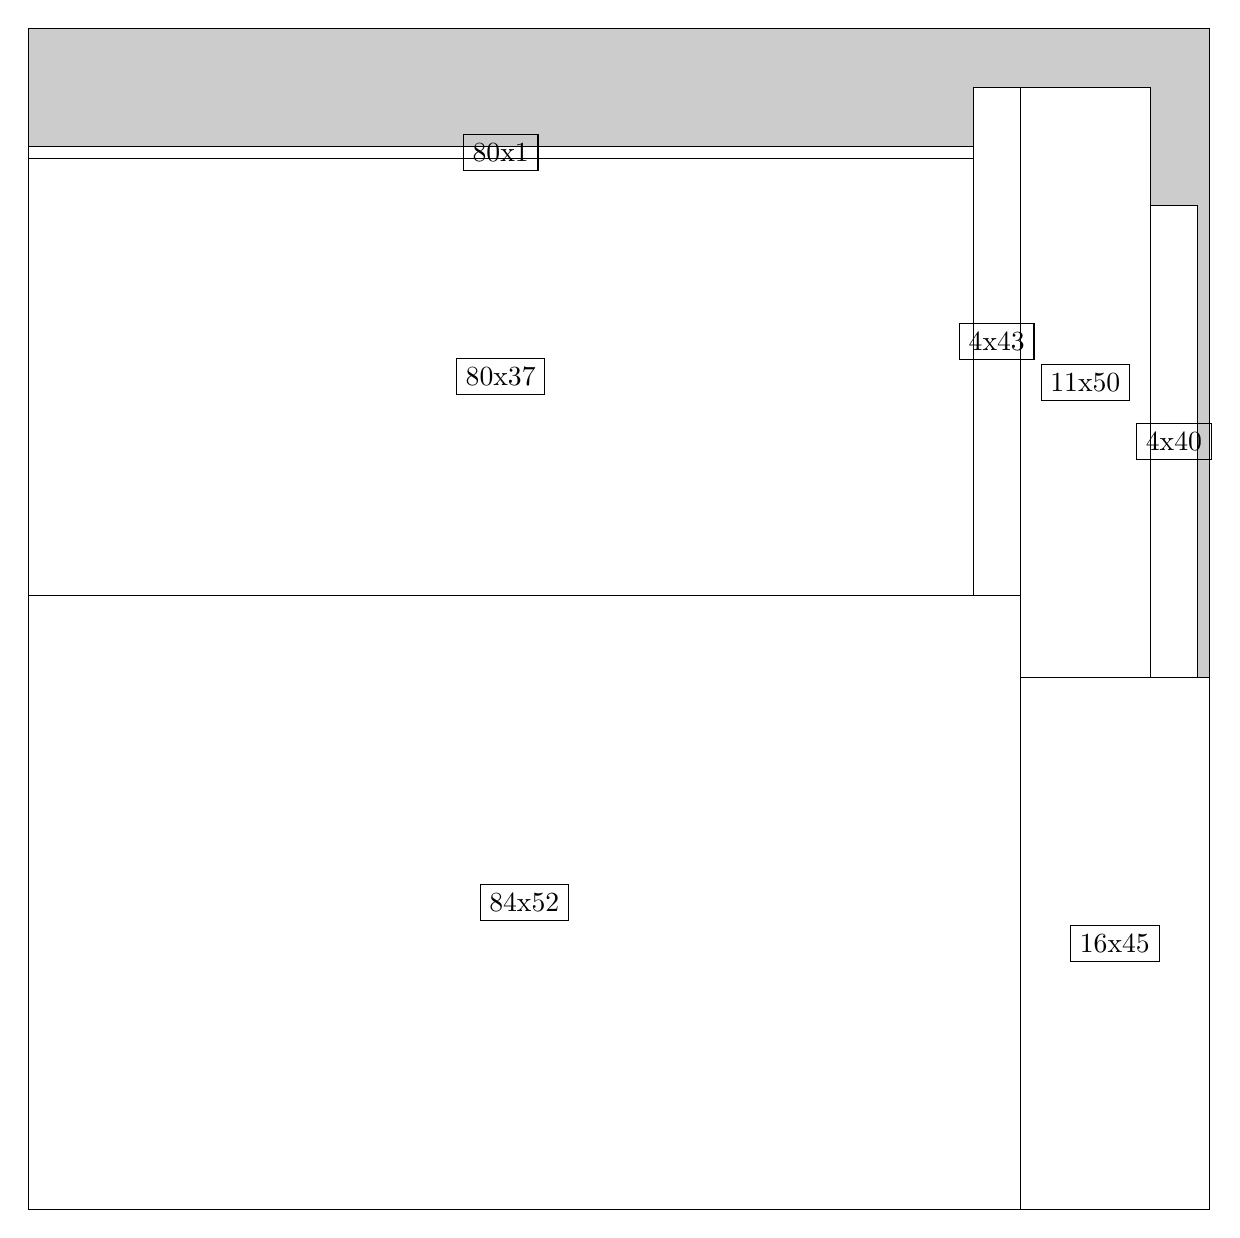
\begin{tikzpicture}[shorten >=1pt,scale=1.0,every node/.style={scale=1.0},->]
\tikzstyle{vertex}=[circle,fill=black!25,minimum size=14pt,inner sep=0pt]
\filldraw[fill=gray!40!white, draw=black] (0,0) rectangle (15.0,15.0);
\foreach \name/\x/\y/\w/\h in {84x52/0.0/0.0/12.6/7.8,80x37/0.0/7.8/12.0/5.55,16x45/12.6/0.0/2.4/6.75,11x50/12.6/6.75/1.65/7.5,4x43/12.0/7.8/0.6/6.45,4x40/14.25/6.75/0.6/6.0,80x1/0.0/13.35/12.0/0.15}
\filldraw[fill=white!40!white, draw=black] (\x,\y) rectangle node[draw] (\name) {\name} ++(\w,\h);
\end{tikzpicture}


w =84 , h =52 , x =0 , y =0 , v =4368
\par
w =80 , h =37 , x =0 , y =52 , v =2960
\par
w =16 , h =45 , x =84 , y =0 , v =720
\par
w =11 , h =50 , x =84 , y =45 , v =550
\par
w =4 , h =43 , x =80 , y =52 , v =172
\par
w =4 , h =40 , x =95 , y =45 , v =160
\par
w =80 , h =1 , x =0 , y =89 , v =80
\par
\newpage


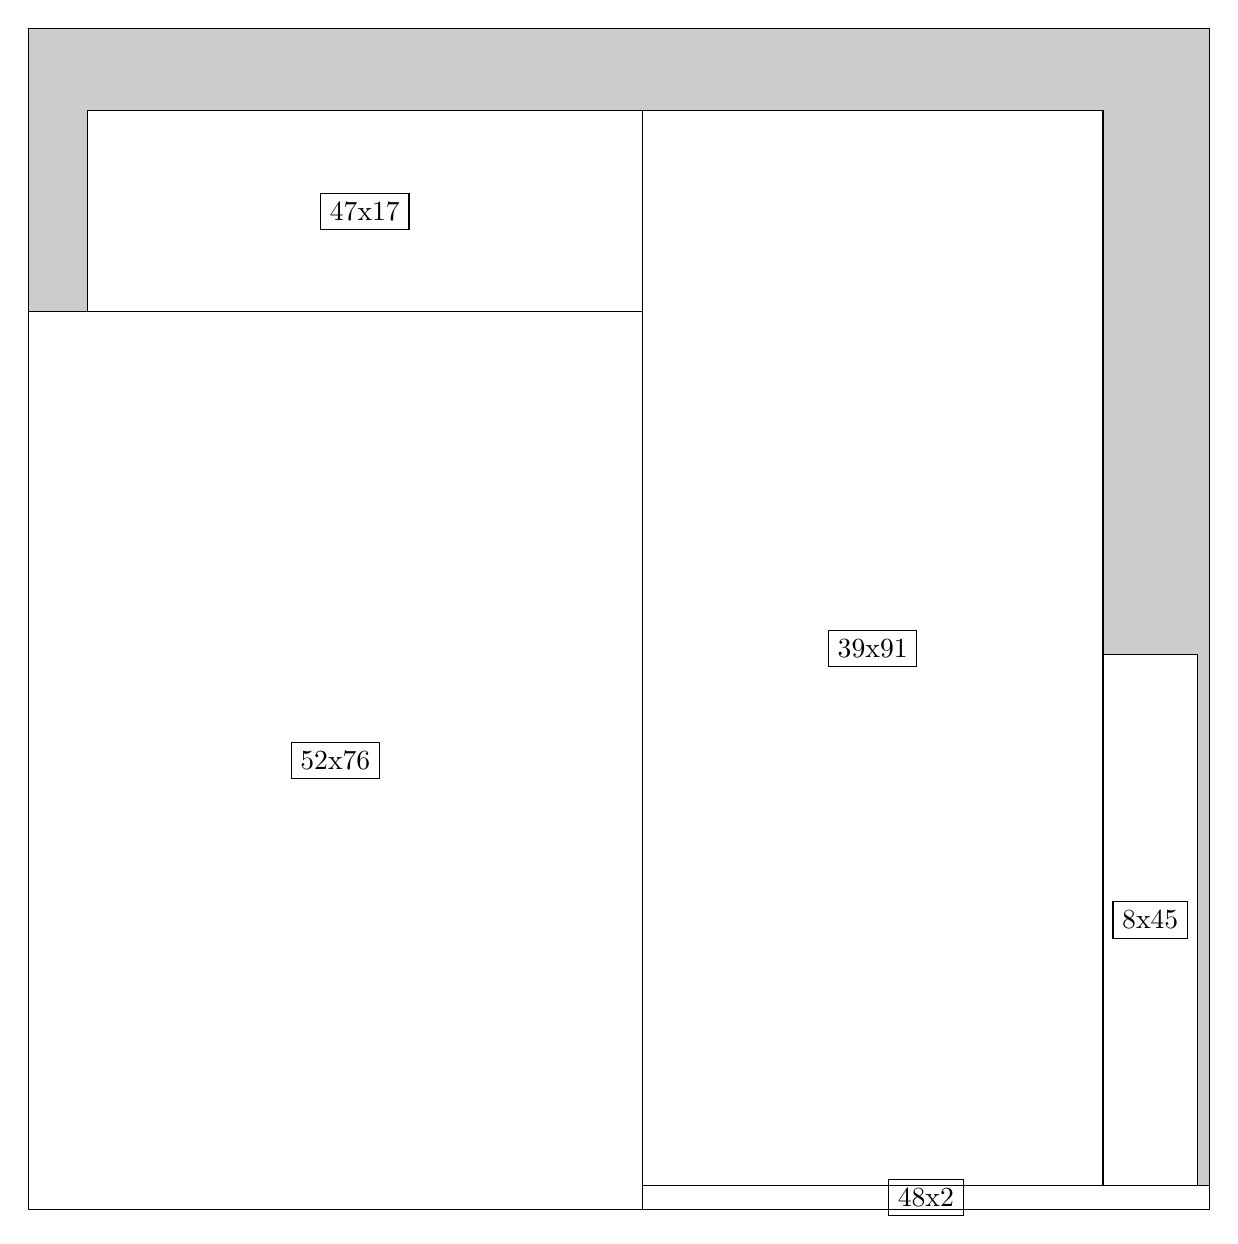
\begin{tikzpicture}[shorten >=1pt,scale=1.0,every node/.style={scale=1.0},->]
\tikzstyle{vertex}=[circle,fill=black!25,minimum size=14pt,inner sep=0pt]
\filldraw[fill=gray!40!white, draw=black] (0,0) rectangle (15.0,15.0);
\foreach \name/\x/\y/\w/\h in {52x76/0.0/0.0/7.8/11.4,39x91/7.8/0.3/5.85/13.65,47x17/0.75/11.4/7.05/2.55,8x45/13.65/0.3/1.2/6.75,48x2/7.8/0.0/7.199999999999999/0.3}
\filldraw[fill=white!40!white, draw=black] (\x,\y) rectangle node[draw] (\name) {\name} ++(\w,\h);
\end{tikzpicture}


w =52 , h =76 , x =0 , y =0 , v =3952
\par
w =39 , h =91 , x =52 , y =2 , v =3549
\par
w =47 , h =17 , x =5 , y =76 , v =799
\par
w =8 , h =45 , x =91 , y =2 , v =360
\par
w =48 , h =2 , x =52 , y =0 , v =96
\par
\newpage


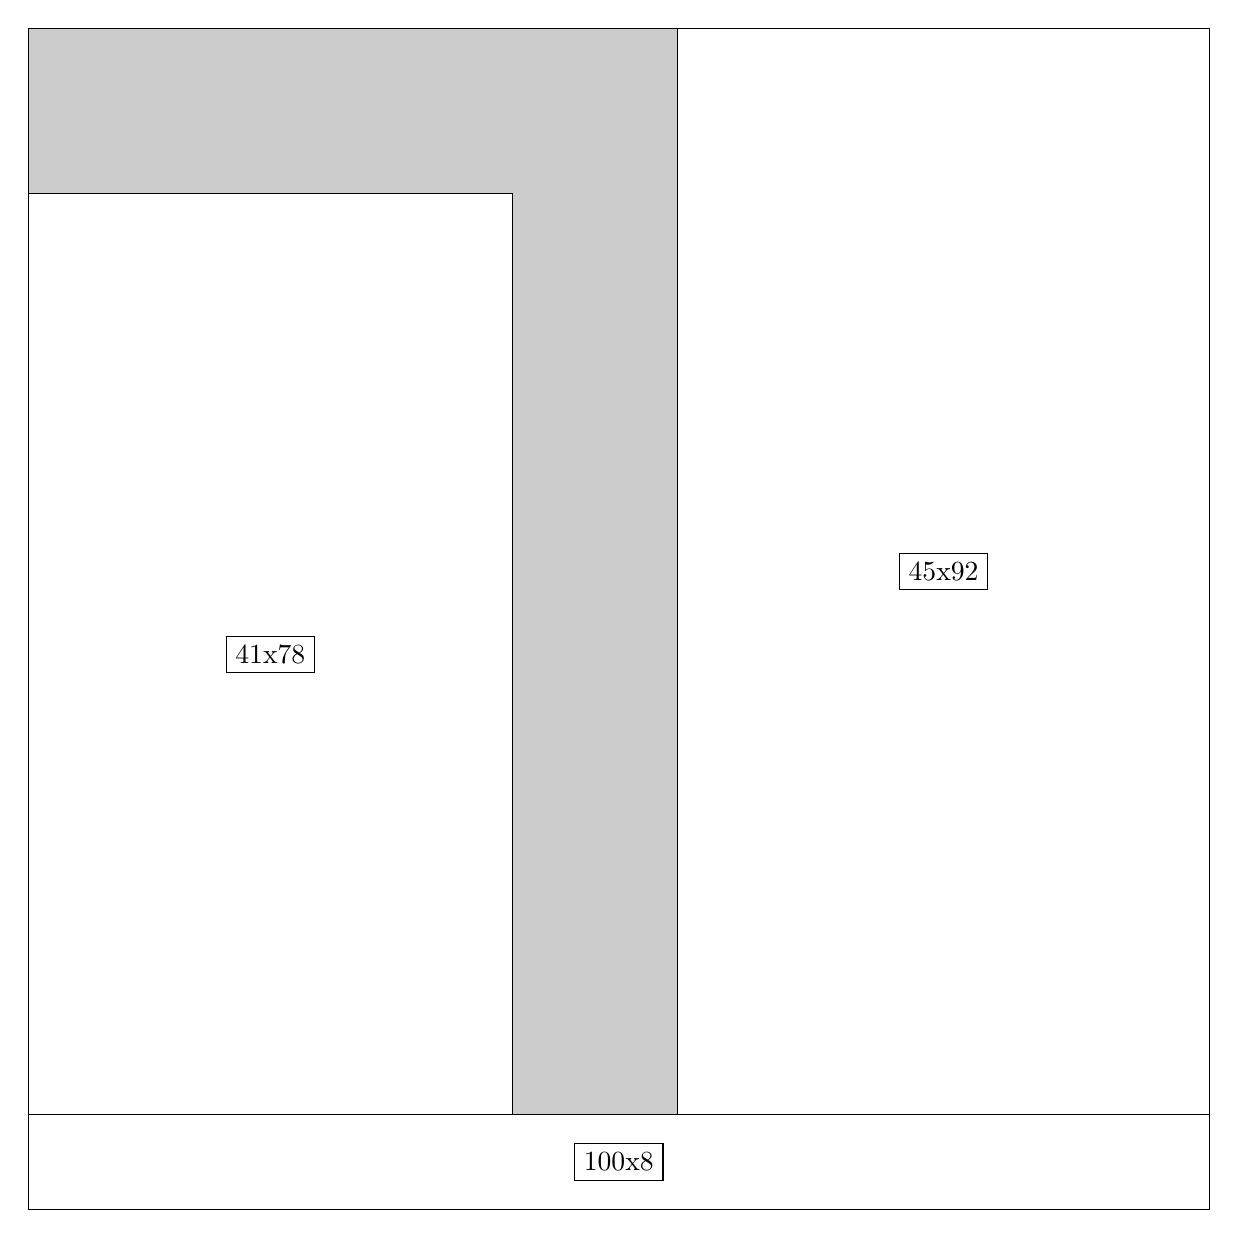
\begin{tikzpicture}[shorten >=1pt,scale=1.0,every node/.style={scale=1.0},->]
\tikzstyle{vertex}=[circle,fill=black!25,minimum size=14pt,inner sep=0pt]
\filldraw[fill=gray!40!white, draw=black] (0,0) rectangle (15.0,15.0);
\foreach \name/\x/\y/\w/\h in {45x92/8.25/1.2/6.75/13.799999999999999,41x78/0.0/1.2/6.1499999999999995/11.7,100x8/0.0/0.0/15.0/1.2}
\filldraw[fill=white!40!white, draw=black] (\x,\y) rectangle node[draw] (\name) {\name} ++(\w,\h);
\end{tikzpicture}


w =45 , h =92 , x =55 , y =8 , v =4140
\par
w =41 , h =78 , x =0 , y =8 , v =3198
\par
w =100 , h =8 , x =0 , y =0 , v =800
\par
\newpage


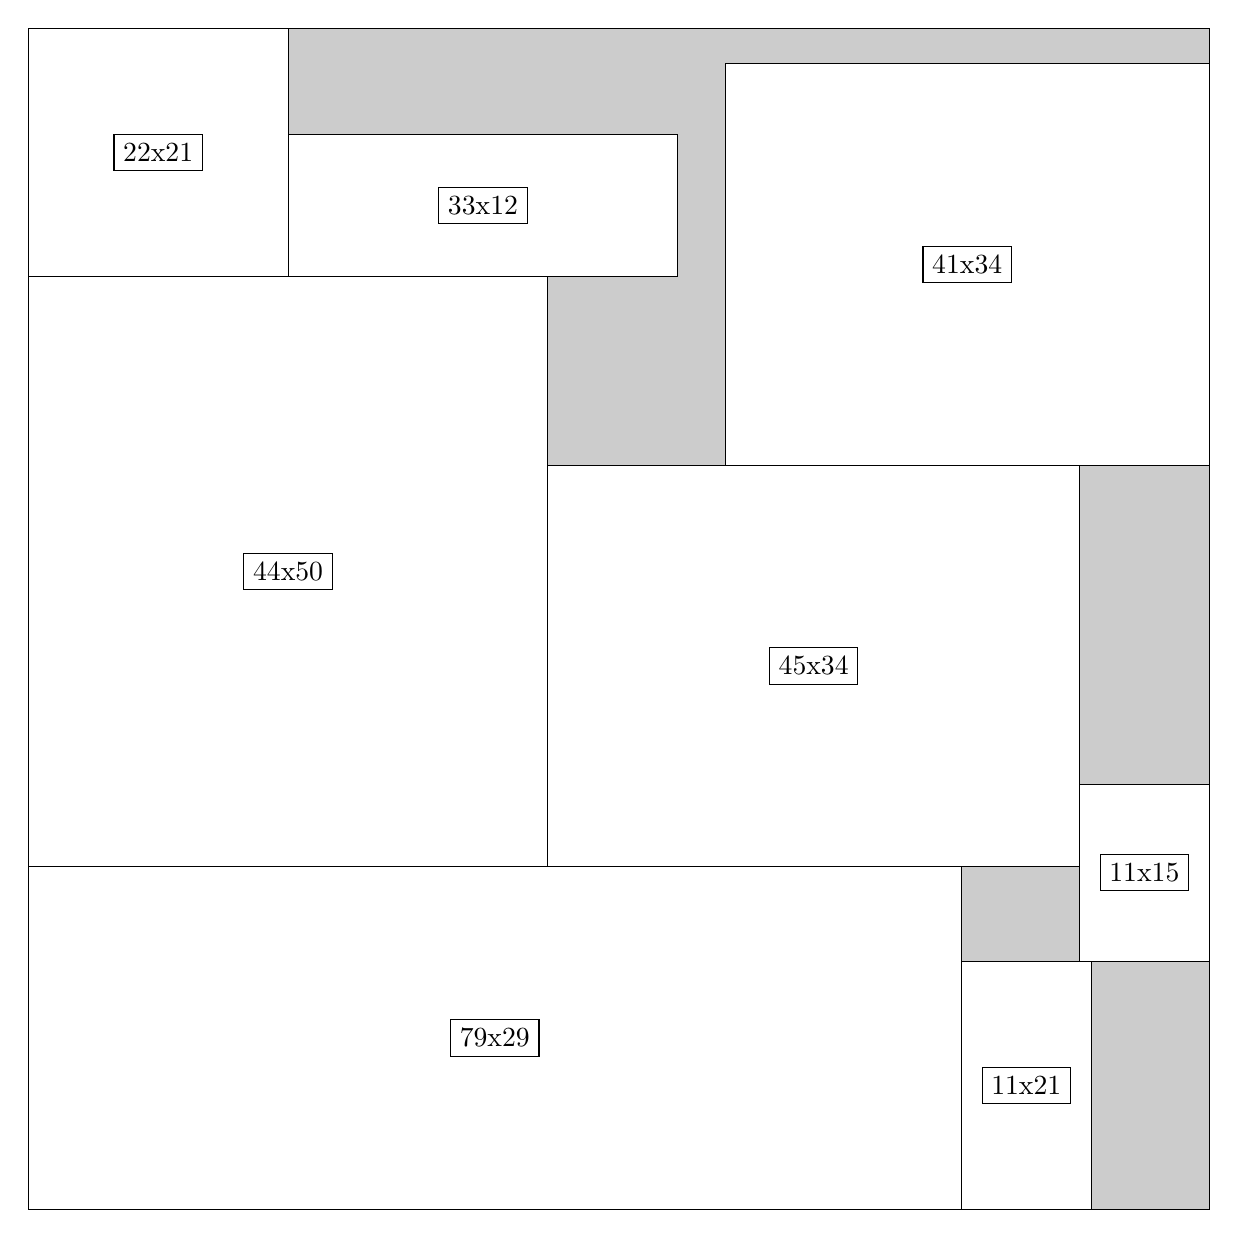
\begin{tikzpicture}[shorten >=1pt,scale=1.0,every node/.style={scale=1.0},->]
\tikzstyle{vertex}=[circle,fill=black!25,minimum size=14pt,inner sep=0pt]
\filldraw[fill=gray!40!white, draw=black] (0,0) rectangle (15.0,15.0);
\foreach \name/\x/\y/\w/\h in {79x29/0.0/0.0/11.85/4.35,44x50/0.0/4.35/6.6/7.5,45x34/6.6/4.35/6.75/5.1,41x34/8.85/9.45/6.1499999999999995/5.1,22x21/0.0/11.85/3.3/3.15,33x12/3.3/11.85/4.95/1.7999999999999998,11x21/11.85/0.0/1.65/3.15,11x15/13.35/3.15/1.65/2.25}
\filldraw[fill=white!40!white, draw=black] (\x,\y) rectangle node[draw] (\name) {\name} ++(\w,\h);
\end{tikzpicture}


w =79 , h =29 , x =0 , y =0 , v =2291
\par
w =44 , h =50 , x =0 , y =29 , v =2200
\par
w =45 , h =34 , x =44 , y =29 , v =1530
\par
w =41 , h =34 , x =59 , y =63 , v =1394
\par
w =22 , h =21 , x =0 , y =79 , v =462
\par
w =33 , h =12 , x =22 , y =79 , v =396
\par
w =11 , h =21 , x =79 , y =0 , v =231
\par
w =11 , h =15 , x =89 , y =21 , v =165
\par
\newpage


\end{document}